% Portada editable de la colección; fotografía original extraída del PDF aportado.
\newcommand{\studiumcover}[3]{\hypersetup{pageanchor=false}\begin{titlepage}\thispagestyle{empty}
\begin{tikzpicture}[remember picture,overlay,x=1pt,y=-1pt]
\begin{scope}[shift={(current page.north west)}]
\clip (0,0) rectangle (595.276,841.89);
\node[inner sep=0pt] at (297.638,420.945){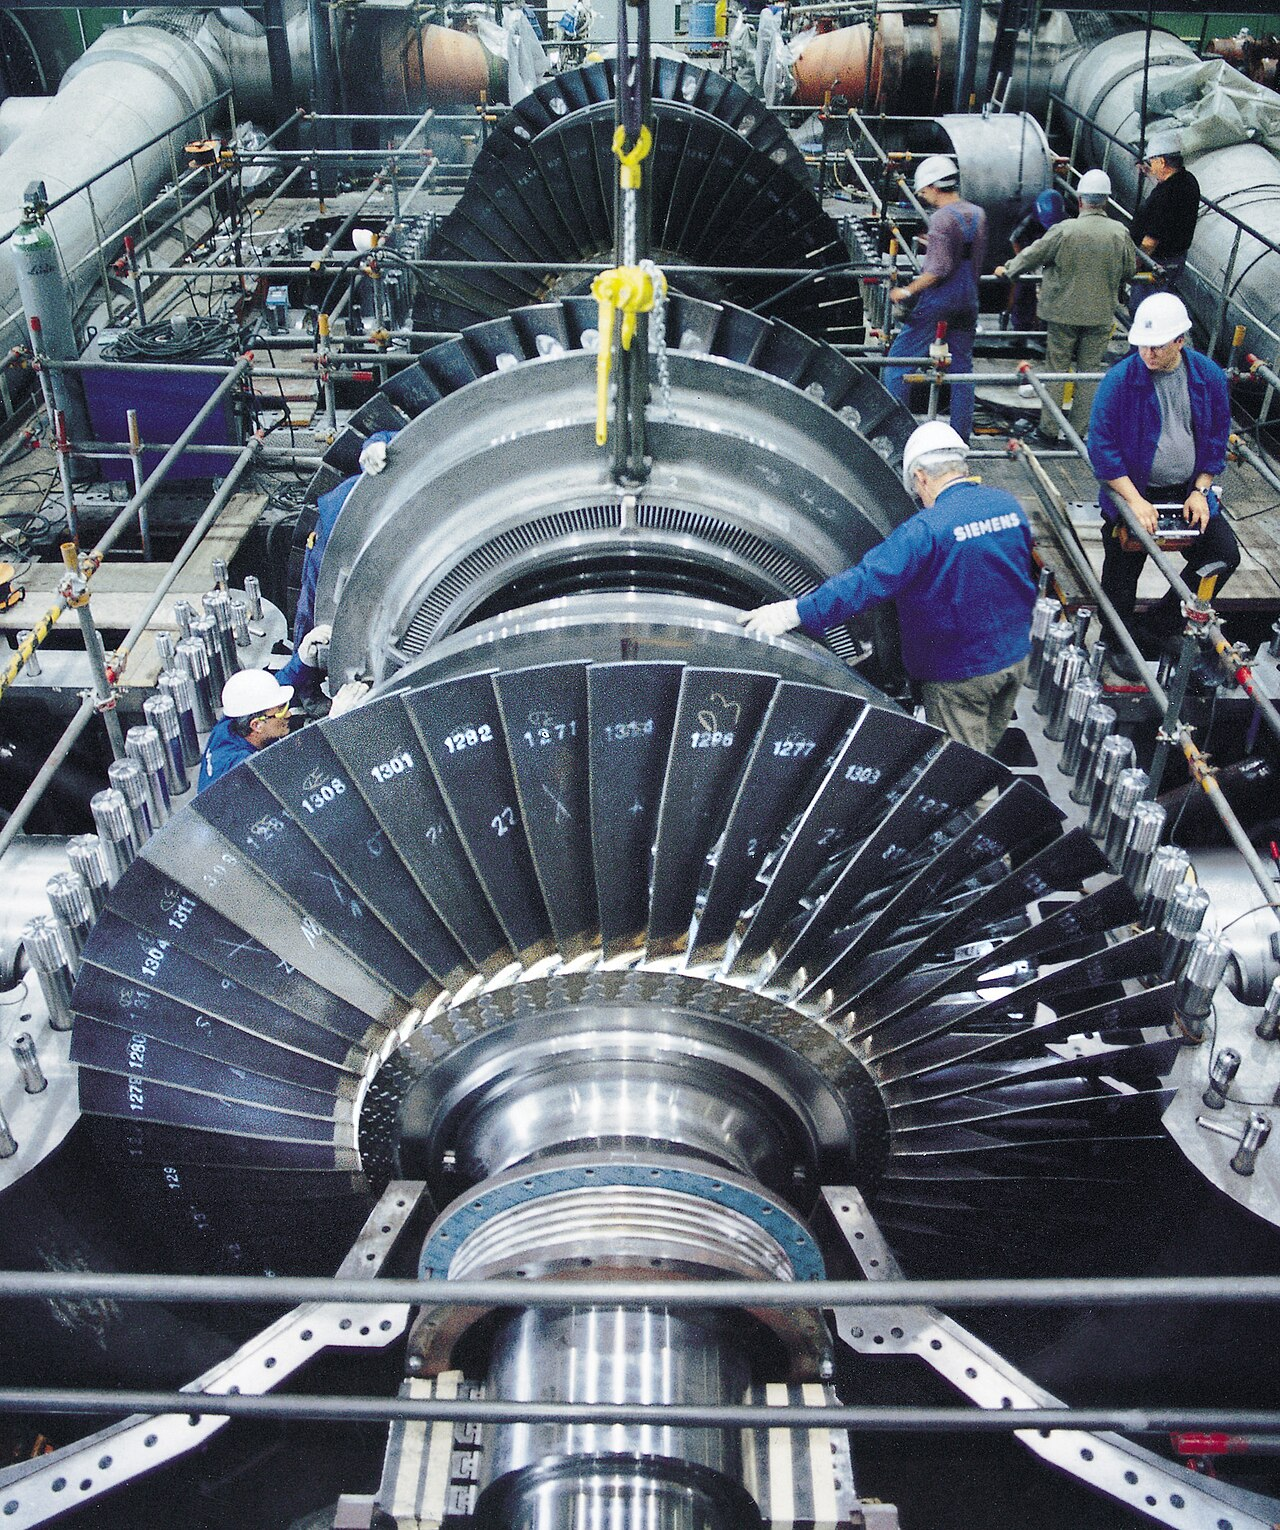
\includegraphics[height=\paperheight]{../figures/cover.jpeg}};
\fill[white,opacity=.91] (0,0) rectangle (595.276,89.5);
\fill[fill={rgb,255:red,14;green,40;blue,55},opacity=.96] (0,585.5) rectangle (595.276,841.89);
\node[anchor=west,text={rgb,255:red,14;green,40;blue,55},font=\sffamily\bfseries\fontsize{18}{21}\selectfont,inner sep=0pt] at (51.223,38.5){STUDIUM};
\draw[draw={rgb,255:red,0;green,182;blue,205},line width=2pt] (51.223,62.5)--(72,62.5);
\node[anchor=west,text={rgb,255:red,14;green,40;blue,55},font=\sffamily\fontsize{8}{10}\selectfont,inner sep=0pt] at (89,65.5){BIBLIOTECA DE INGENIERÍA};
\node[anchor=west,text={rgb,255:red,0;green,195;blue,213},font=\sffamily\fontsize{10}{12}\selectfont,inner sep=0pt] at (51.223,608){#3};
\node[anchor=north west,text=white,text width=493pt,align=left,font=\rmfamily\bfseries\fontsize{33}{36}\selectfont,inner sep=0pt] at (51.223,631){#1};
\node[anchor=north west,text=white,text width=490pt,align=left,font=\sffamily\fontsize{10}{13}\selectfont,inner sep=0pt] at (51.223,718){#2};
\node[anchor=west,text=white,font=\sffamily\bfseries\fontsize{10}{12}\selectfont,inner sep=0pt] at (51.223,758){GRADO EN INGENIERÍA AEROESPACIAL};
\node[anchor=west,text=white,font=\sffamily\fontsize{10}{12}\selectfont,inner sep=0pt] at (51.223,773){Universidad de León};
\draw[white,opacity=.35,line width=.5pt] (51.223,786)--(544.05,786);
\node[anchor=west,text=white,font=\sffamily\fontsize{10}{12}\selectfont,inner sep=0pt] at (51.223,810){2026};
\node[anchor=east,text=white,font=\sffamily\bfseries\fontsize{10}{12}\selectfont,inner sep=0pt] at (544.05,810){I Edición};
\end{scope}\end{tikzpicture}\null\end{titlepage}\hypersetup{pageanchor=true}}
